\documentclass{beamer}

\usepackage{beamerthemesplit}
\usepackage[spanish,activeacute]{babel}
\usepackage[utf8]{inputenc}
\usepackage{graphicx}

\begin{document}
\title{Solución exacta de problemas difíciles: Backtraking para ``Satisfiability"}
\author{Daniel Izquierdo}
\date{25 de noviembre de 2008}

\frame{\titlepage}

\section[Contenido]{}
\frame
{
  \begin{itemize}
  \item Definición del problema.
  \item Opciones para resolver el problema.
  \item Técnicas para mejorar backtracking.
  \end{itemize}
}

\section{Introducción}

\frame
{
  \frametitle{Ejemplos}

  Problema de satisfactibilidad: ¿es posible satisfacer las siguientes expresiones?

  \begin{itemize}
  \item $v_1 \vee v_2$
  \item $(v_1 \vee \neg v_2) \wedge (v_2 \vee v_3)$
  \item $(v_1 \wedge \neg v_2) \wedge (v_2 \wedge v_3)$
  \end{itemize}
}

\frame
{
  \frametitle{Un ejemplo más complicado}

  \begin{itemize}
  \item $(\neg v_{1} \vee v_5 \vee v_3) \wedge (\neg v_{3} \vee \neg v_{4} \vee \neg v_{6}) \wedge (\neg v_{1} \vee \neg v_{8} \vee v_{7}) \wedge$
        $(\neg v_{4} \vee \neg v_{1} \vee v_{5}) \wedge (v_4 \vee v_2 \vee v_8) \wedge (\neg v_3 \vee \neg v_9 \vee v_1) \wedge (v_7 \vee v_4 \vee v_8)$
  \end{itemize}
}

\frame
{
  \frametitle{CNF}

  \begin{itemize}
  \item CNF: ``Conjunctive normal form'' o ``Forma normal conjuntiva''
  \item Es una forma ``estándar'' de representar fórmulas.
  \item La CNF de una fórmula consiste en una conjunción de disyunciones $(A \vee B \vee \ldots) \wedge (C \vee D \vee \ldots) \wedge \ldots$
  \item Cualquier expresión proposicional se puede convertir a CNF preservando
        equivalencia o satisfactibilidad.
  \item Cada elemento de la conjunción de una fórmula CNF se denomina cláusula.
  \end{itemize}
}

\frame
{
  \frametitle{¿Cuál es el problema y cómo resolverlo?}

  Dada una fórmula $F$ en CNF con $n$ variables $X_1, \ldots, X_n$, decir si es
  posible asignar valores a las variables de manera que $F$ se satisfaga.

  Enfoques:

  \begin{itemize}
  \item Algoritmos probabilísticos
  \item Backtracking
  \end{itemize}
}

\section{Backtracking}

\frame
{
  \frametitle{Enfoque ``fuerza bruta''}

  Usar backtracking para intentar todas las posibles asignaciones de valores a variables. Por
  ejemplo, para dos variables $X$ e $Y$ podemos probar:

  $$
  (X=0,Y=0), (X=0,Y=1), (X=1,Y=0), (X=1,Y=1)
  $$

  Problema con este enfoque: toma tiempo exponencial ($2^n$)
}

\frame
{
  \frametitle{BCP}

  \begin{itemize}
   \item BCP: ``Boolean Constraint Propagation'' o ``Propagación de restricciones booleanas''
   \item Al realizar una asignación puedo deducir sus efectos: cláusulas satisfechas, cláusulas unitarias y conflictos.
   \item Ejemplo 1: $(X \vee Y) \wedge (\neg X \vee \neg W) \wedge (W \vee U)$
   \item Ejemplo 2: $(X \vee Y) \wedge (X \vee Z) \wedge (\neg X \vee \neg W) \wedge (W)$
  \end{itemize}
}

\frame
{
  \frametitle{Exploración del espacio de búsqueda}

  Exploramos un ``árbol de decisiones'' y utilizamos técnicas
  para incrementar la velocidad de la exploración. Un nodo del árbol
  de decisiones representa una asignación a una variable no asignada.
  Proceso:

  \begin{enumerate}
   \item Tomo una decisión de asignación.
   \item ``Extiendo'' el conjunto de asignaciones actual (BCP).
   \item Si no pude satisfacer la fórmula, me retracto de la decisión de
         asignación tomada para intentar otra asignación (backtracking).
  \end{enumerate}
}

\frame
{
  \frametitle{Heurísticas para la decisión de asignación}

  \begin{itemize}
   \item Se pueden utilizar heurísticas para intentar tomar una buena decisión de asignación.
   \item Ejemplo (GRASP): elegir la asignación que satisface el mayor número de cláusulas.
  \end{itemize}
}

\frame
{
  \frametitle{Análisis de conflictos}

  Podemos ir más allá de BCP y averiguar sobre las causas de los conflictos,
  aprovechando esta información para optimizar la búsqueda.

  \begin{enumerate}
   \item Aprendizaje
   \item Backtracking no cronológico
  \end{enumerate}

}

\frame
{
  \frametitle{Aprendizaje}

   \begin{itemize}
    \item Podemos agregar cláusulas nuevas a partir de un conflicto para evitar conseguirlo de nuevo.
    \item Se puede emplear una heurística para decidir si agregar cada cláusula o no, de manera de no
          aumentar demasiado el tamaño de la base de datos.
   \end{itemize}
}

\frame
{
  \frametitle{Aprendizaje (cont.)}

  \scalebox{0.3}{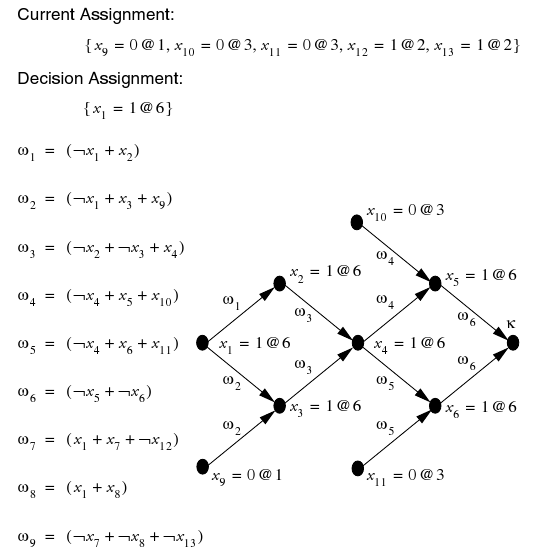
\includegraphics{ig.png}}

  Podemos agregar $(\neg X_1 \vee X_9 \vee X_10 \vee X_11)$.
}

\frame
{
  \frametitle{Backtracking no cronológico}

   \begin{itemize}
    \item Al conseguir un conflicto, podemos hacer backtracking más allá de un nivel en el
          árbol de decisiones.
   \end{itemize}
}

\frame
{
  \frametitle{Backtracking no cronológico (cont.)}

  \scalebox{0.3}{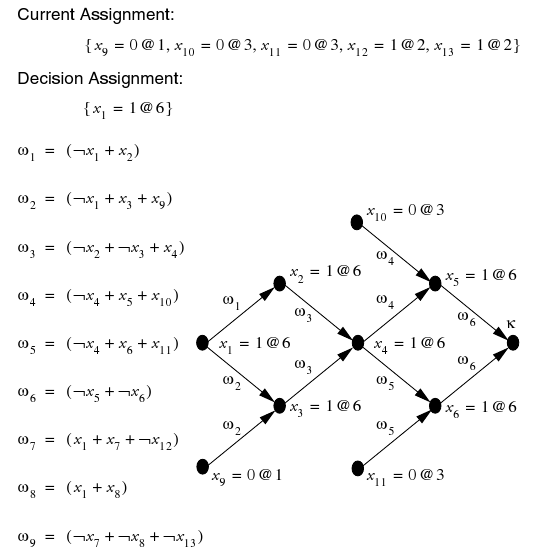
\includegraphics{ig.png}}

  Podemos regresar al nivel 3 del árbol de decisiones.
}

\section{Preguntas}

\frame
{
  \frametitle{Preguntas}
}

\end{document}
